% =====================================================================
%  UCS762 Cybersecurity for Mobility Systems - Individual Assignment
%  Springer LNCS format (llncs class, available on Overleaf by default)
%  Replace the author block and the GitHub URL (search for "TODO").
% =====================================================================
\documentclass[runningheads]{llncs}

\usepackage[T1]{fontenc}
\usepackage{lmodern}
\usepackage{graphicx}
\usepackage{microtype}
\usepackage{booktabs}
\usepackage{amsmath,amssymb}
\usepackage{tikz}
\usetikzlibrary{arrows.meta,positioning,fit,calc}
\usepackage{xcolor}
\usepackage[hidelinks]{hyperref}
\usepackage{url}
\usepackage{pifont}
\newcommand{\cmark}{\ding{51}}
\newcommand{\xmark}{\ding{55}}
\newcommand{\pmark}{$\circ$}
\renewcommand\UrlFont{\color{blue!60!black}\rmfamily}

\begin{document}

\title{CANtinel: Verifying In-Vehicle CAN Security Problems and Overcoming the Limits of Market Intrusion Detection Tools with an Open, Explainable IDS/IPS}
\titlerunning{CANtinel: An Open, Explainable IDS/IPS for In-Vehicle CAN}

% Author details
\author{Atishay Kashyap\inst{1}}
\authorrunning{A. Kashyap}
\institute{Department of Computer Science and Engineering,\\
Thapar Institute of Engineering and Technology, Patiala, Punjab, India\\
\email{akashyap1\_be23@thapar.edu}\\
Roll No.: 102303859 \quad Course: UCS762 Cybersecurity for Mobility Systems}

\maketitle

\begin{abstract}
The Controller Area Network (CAN) that links a vehicle's electronic control units (ECUs) has no sender
authentication, no encryption and a priority arbitration that any node can abuse. We first \emph{verify} these
problems on a simulated 24-ID vehicle network, where one flooding node starves 15 of the 24 message IDs, and show why
market tools leave a gap: commercial IDPS products are closed, IT IDSs do not understand CAN, and deep-learning
detectors need labelled attacks and give no explanation. Our open-source framework \textbf{CANtinel} combines an ID whitelist, a
\emph{phase-locked} timing model of every ECU's schedule, payload semantics learned without a DBC file, cross-layer
fusion with self-tuning, a filtering gateway and SecOC-lite authentication. Over five vehicles and seven attack classes
it reaches a frame-level F1 of 0.96--1.00 on all flooding, spoofing, replay and naive masquerade attacks at a
false-positive rate of $2.3\times10^{-6}$, beats interval and entropy baselines (F1 0.999 vs.\ 0.000 on masquerade),
and its SecOC-lite layer rejects every replayed, forged and stealth-masquerade frame.
\keywords{Automotive cybersecurity \and CAN bus \and Intrusion detection and prevention \and SecOC \and ISO/SAE 21434 \and AIS-189.}
\end{abstract}

% ---------------------------------------------------------------------
\section{Introduction}
% ---------------------------------------------------------------------
Dozens of ECUs in a modern car communicate over CAN, whose frames carry no sender address, reach
every node, win arbitration by lowest identifier and have no integrity protection. Telematics, infotainment, OBD-II
dongles and over-the-air updates now connect this once-isolated bus to the outside world. Attackers on the bus can disable brakes and control
the engine~\cite{koscher2010}, reach it remotely through cellular and media interfaces~\cite{checkoway2011}, and
compromise unmodified vehicles over the Internet, as the Jeep Cherokee hack that led to a recall of 1.4 million
vehicles showed~\cite{miller2015}. Upstream's 2026 report counted 494 public automotive and smart-mobility incidents in
2025, 92\,\% of them remote and 44\,\% involving ransomware~\cite{upstream2026}.

UN R155/R156 now require cyber security and software update management systems~\cite{unr155}, ISO/SAE 21434
defines the engineering process~\cite{iso21434}, and India's AIS-189/AIS-190 are proposed to become mandatory from
1 October 2026, first for new models with Level~3 automation or above~\cite{ais189}. All expect attacks in the field to
be detected and handled.

\textbf{Problem.} Commercial CAN intrusion detection is closed and licensed to OEMs; researchers, fleets, EV
start-ups and auditors lack a transparent tool they can inspect and adapt, and open alternatives ignore CAN semantics or
need labelled attacks.

\textbf{Contributions.} We review the literature and market tools (Sect.~\ref{sec:lit}), verify the core CAN
weaknesses experimentally (Sect.~\ref{sec:verify}), design the open IDS/IPS CANtinel (Sect.~\ref{sec:design}) and
evaluate it on seven attack classes, including masquerade attacks that most public datasets lack (Sect.~\ref{sec:eval}). The code is at \url{https://github.com/AtishayKashyap/cantinel}.

% ---------------------------------------------------------------------
\section{Background and Literature Review}\label{sec:lit}
% ---------------------------------------------------------------------
\textbf{CAN attack surface.} A CAN frame has an 11-bit identifier, a data length code (DLC) and up to 8 data bytes;
most messages are periodic (10--1000\,ms) and often carry a rolling counter and a checksum. Attackers enter through
OBD-II, telematics or infotainment ECUs~\cite{checkoway2011} and perform \emph{denial of service} (flooding high-priority IDs), \emph{fuzzing},
\emph{spoofing}, \emph{replay} or \emph{masquerade}, in which the genuine ECU is silenced, e.g.\ by the bus-off
attack~\cite{cho2016busoff}, and impersonated at the correct period.

\textbf{Intrusion detection.} Surveys~\cite{wu2020survey} distinguish timing, statistical and payload/ML detectors.
Song et al.~\cite{song2016} detect injections from shortened inter-arrival times, and Cho and Shin~\cite{cho2016cids}
fingerprint ECUs by clock skew. Müter and Asaj~\cite{muter2011} monitor identifier entropy. Payload detectors use deep neural networks~\cite{kang2016}, convolutional networks~\cite{song2020} or unsupervised
recurrent models~\cite{hanselmann2020}.
The popular HCRL Car-Hacking dataset injects DoS, fuzzy and spoofed gear/RPM frames every
0.3, 0.5 and 1\,ms~\cite{song2020}. Verma et al.~\cite{verma2024road} find public datasets limited to simple injection
attacks and release ROAD with stealthier, including masquerade, attacks, and Longari et al.~\cite{longari2025canter} show that drop-and-spoof
attacks evade current IDSs. High scores on flooding data therefore say little about stealthy attacks.

\textbf{Authentication.} vatiCAN~\cite{nurnberger2016} adds MACs and freshness to CAN; industry uses AUTOSAR
SecOC~\cite{autosar_secoc}, which appends a truncated freshness value (FV) and MAC to each protected PDU.

\textbf{Market tools and their gaps.} Table~\ref{tab:market} compares tools by publicly documented properties.
PlaxidityX (formerly Argus, part of Continental's Elektrobit) offers a CAN IDPS that monitors traffic and prevents
attacks such as DoS and brute force~\cite{plaxidityx}. ETAS's ESCRYPT CycurIDS combines known attack patterns with
comparison against expected communication, and CycurGATE is an in-vehicle firewall~\cite{etas}. Upstream runs a
cloud-based vehicle SOC that analyses fleet data~\cite{upstream2026}. These products are mature but closed and built
for OEM series projects, so their logic cannot be inspected or reproduced; IT IDSs such as Snort ignore CAN semantics.

\begin{table}[t]
\centering
\caption{Market and research tools versus the needs of an open CAN IDS
(\cmark\ yes, \xmark\ no, \pmark\ partly / not publicly documented).}\label{tab:market}
\scriptsize
\setlength{\tabcolsep}{3pt}
\begin{tabular}{@{}lccccc@{}}
\toprule
Requirement & \shortstack{Commercial\\IDPS~\cite{plaxidityx,etas}} & \shortstack{Cloud\\VSOC~\cite{upstream2026}} & \shortstack{IT IDS\\(Snort etc.)} & \shortstack{Academic\\DL IDS} & \shortstack{CANtinel\\(ours)}\\
\midrule
Open source / auditable logic       & \xmark & \xmark & \cmark & \pmark & \cmark\\
Understands CAN timing \& payload   & \cmark & \cmark & \xmark & \cmark & \cmark\\
Works without OEM DBC files         & \pmark & \pmark & --     & \cmark & \cmark\\
No labelled attack data needed      & \pmark & \pmark & \xmark & \xmark & \cmark\\
Explainable, per-frame alerts       & \pmark & \pmark & \cmark & \xmark & \cmark\\
In-line prevention (gateway)        & \cmark & \xmark & \pmark & \xmark & \cmark\\
Message authentication (SecOC)      & \pmark & \xmark & \xmark & \xmark & \cmark\\
Free for research / small fleets    & \xmark & \xmark & \cmark & \cmark & \cmark\\
\bottomrule
\end{tabular}
\end{table}

% ---------------------------------------------------------------------
\section{Verifying the Security Problems}\label{sec:verify}
% ---------------------------------------------------------------------
\textbf{Threat model.} The attacker controls one node on the bus (compromised ECU or malicious OBD-II device), can read
all frames, send any identifier at any rate and silence another ECU with a bus-off attack~\cite{cho2016busoff}, but
cannot extract keys from an ECU's hardware security module.

\textbf{Setup.} Our discrete-event simulator models eight ECUs sending 24 IDs (23 periodic) over a 500\,kbit/s bus
with bit-accurate frame lengths, priority arbitration, transmit mailboxes, clock drift and jitter. Payloads follow a
realistic drive and contain XOR, SUM and CRC-8 checksums and counters; IDs 0x316 (RPM) and 0x43F (gear) mirror
HCRL~\cite{song2020}.

\textbf{Findings.} (i)~Nothing in a frame identifies its sender, so any node can send any ID.
(ii)~A DoS node sending ID~0x000 every 0.3\,ms drives the bus to 100\,\% load, halves legitimate throughput and
\emph{starves 15 of the 24 IDs} (14 completely), including vehicle speed, gear, RPM and airbag status.
(iii)~A node spoofing RPM every 1\,ms outnumbers the genuine ECU 10:1, so receivers show the attacker's value about
91\,\% of the time. (iv)~Recorded frames can be replayed verbatim.

% ---------------------------------------------------------------------
\section{Proposed Solution: CANtinel}\label{sec:design}
% ---------------------------------------------------------------------
CANtinel (Fig.~\ref{fig:arch}) learns a \emph{vehicle profile} from attack-free traffic, without a DBC file or attack
labels, stores it as readable JSON and processes frames online. Every alert names the layer, the rule and the observed
versus expected value.

\begin{figure}[t]
\centering
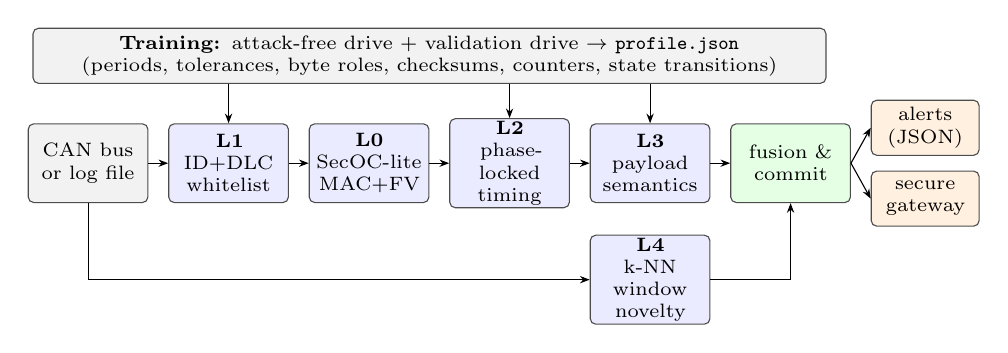
\begin{tikzpicture}[
  font=\scriptsize, >={Stealth[length=3.5pt]}, node distance=2.5mm,
  box/.style={draw=black!70, rounded corners=2pt, align=center, minimum height=10mm, text width=14.5mm, inner sep=1pt, fill=white},
  lay/.style={box, fill=blue!8},
  io/.style={box, fill=black!5},
  outb/.style={box, fill=orange!12, minimum height=7mm, text width=13mm}]
\node[io] (bus) {CAN bus\\ or log file};
\node[lay, right=of bus] (l1) {\textbf{L1}\\ ID{+}DLC\\ whitelist};
\node[lay, right=of l1] (l0) {\textbf{L0}\\ SecOC-lite\\ MAC{+}FV};
\node[lay, right=of l0] (l2) {\textbf{L2}\\ phase-locked\\ timing};
\node[lay, right=of l2] (l3) {\textbf{L3}\\ payload\\ semantics};
\node[box, right=of l3, fill=green!10] (fu) {fusion \&\\ commit};
\node[outb, right=of fu, yshift=4.5mm] (al) {alerts\\ (JSON)};
\node[outb, right=of fu, yshift=-4.5mm] (gw) {secure\\ gateway};
\node[lay, below=4mm of l3] (l4) {\textbf{L4}\\ k-NN window\\ novelty};
\node[io, above=5mm of l0.north east, anchor=south, text width=100mm, minimum height=7mm, execute at begin node=\hyphenpenalty 10000\relax] (tr)
  {\textbf{Training:} attack-free drive + validation drive $\rightarrow$ \texttt{profile.json}\\
   (periods, tolerances, byte roles, checksums, counters, state transitions)};
\draw[->] (bus) -- (l1);
\draw[->] (l1) -- (l0);
\draw[->] (l0) -- (l2);
\draw[->] (l2) -- (l3);
\draw[->] (l3) -- (fu);
\draw[->] (fu.east) -- (al.west);
\draw[->] (fu.east) -- (gw.west);
\draw[->] (bus.south) |- (l4.west);
\draw[->] (l4.east) -| (fu.south);
\foreach \n in {l1,l2,l3} \draw[->] (\n.north |- tr.south) -- (\n.north);
\end{tikzpicture}
\caption{CANtinel architecture. Only frames accepted by all layers update the state of L2 and L3
(cross-layer feedback in the fusion stage).}\label{fig:arch}
\end{figure}

\textbf{L1: Specification.} The learned set of IDs and DLCs is a whitelist; an unknown ID or DLC raises a
high-severity alert, and unknown IDs below the lowest legitimate one are reported as a priority flood.

\textbf{L2: Phase-locked timing.} Interval detectors~\cite{song2016} compare a frame with its \emph{predecessor}, so
an injection makes the next genuine frame look early too. CANtinel instead locks onto each ECU's \emph{schedule}. For an ID with learned period
$T$ it keeps an anchor $r$ (estimated send time of the last accepted frame) and flags a frame arriving at $t$ as early if
$t < r + T - \tau$. When a frame is accepted, with $n=\lfloor (t-r+\tau)/T\rfloor$, $\hat t=r+nT$ and $e=t-\hat t$, an
asymmetric phase-locked loop updates
\begin{equation}
r \leftarrow \hat t + \alpha_{-}e \;(e<0),\qquad r \leftarrow \hat t + \alpha_{+}e \;(0\le e\le\tau),\qquad r\leftarrow\hat t \;(e>\tau),
\end{equation}
with $\alpha_{-}=0.5$ and $\alpha_{+}=0.02$. A genuine ECU can be delayed but is never ahead of its schedule, so the anchor follows the lower envelope of arrivals
and $\tau$ only covers jitter; it is learned on training data, $\tau=\max(1.25|\min e|, 4\sigma_e, 0.01T)$, and is 0.25--1.05\,ms for our 10\,ms
messages. Timing alerts are downgraded while foreign IDs flood the bus, and two payload-valid frames exactly one period apart
with no accepted frame in between re-synchronise the anchor, since an injector beside the real ECU always leaves
accepted genuine frames in between.

\textbf{L3: Payload semantics without a DBC file.} Each payload byte gets a learned role: \emph{checksum} (XOR, SUM or
CRC-8 J1850 of the other bytes in $\ge$99.9\,\% of frames), \emph{counter} (byte or nibble incrementing by one),
\emph{enum} ($\le$16 values, with the observed state-transition graph, e.g.\ gear D2$\leftrightarrow$D3),
\emph{range} (min/max, maximum change per period) or \emph{free}. A frame is compared with the \emph{last accepted} frame of its ID: a checksum mismatch, a counter
advance different from the elapsed periods $\mathrm{round}(\Delta t/T)$, an unseen value or transition, or a
range/rate violation raises an alert.

\textbf{Fusion and self-tuning.} A frame is flagged if any layer raises a high or medium alert, and only frames
accepted by \emph{all} layers update the timing anchor and payload reference. An injected frame that slips into the
timing window with an impossible gear transition thus cannot become the reference. After training, the profile is run on a second attack-free drive; rules that fire are
pruned or extended and tolerances widened, which removes rules that reflect only one drive (fuel level, odometer).

\textbf{L4: Window novelty.} As a safety net, nine features (frame count, unique IDs, ID entropy, unknown-ID fraction,
minimum gap, maximum rate ratio, payload Hamming distance, fraction below the lowest ID, bus load) are computed per
100\,ms window and scored by the mean standardised distance to the 5 nearest attack-free windows. An Isolation Forest is unsuitable: its score saturates outside the training range, giving window F1 0.08 on DoS.

\textbf{Prevention.} The \emph{secure gateway} between domains (e.g.\ infotainment/OBD and powertrain) forwards a
frame only if its ID is whitelisted, the engine raised no high/medium alert and a per-ID token bucket (1.2$\times$ the
learned rate, burst 3) allows it. \emph{SecOC-lite} follows AUTOSAR SecOC~\cite{autosar_secoc}: each protected PDU
carries an 8-bit truncated FV and a 24-bit truncated AES-128-CMAC over $\mathit{DataID}\Vert\mathit{payload}\Vert
\mathit{FV}_{64}$. The receiver reconstructs the full FV, tolerating lost frames, rejects FV jumps above 64 and raises
\texttt{AUTH\_FAIL} alerts, plus \texttt{MAC\_BRUTE\_FORCE} after more than five failures per second. A forgery succeeds with probability $2^{-24}$ per attempt, and every failure is detected.

\textbf{Technology stack.} About 2{,}700 lines of Python~3 (NumPy, scikit-learn, \texttt{cryptography},
python-can for SocketCAN/PCAN/Vector), a CLI and 21 unit tests; \texttt{cantinel benchmark} reproduces all results.

% ---------------------------------------------------------------------
\section{Experimental Evaluation}\label{sec:eval}
% ---------------------------------------------------------------------
\textbf{Protocol.} For each of five simulated vehicles CANtinel is trained on a 300\,s attack-free drive, self-tuned
on a 120\,s drive and tested on 60\,s captures (one clean, one per attack, 4--5 bursts of 3--5\,s as in HCRL). Besides the four HCRL-style attacks we test replay of
steering frames, a \emph{naive masquerade} (silenced speed ECU, attacker patches the speed bytes of a sniffed frame)
and a \emph{stealth masquerade} (the attacker also continues the counter and recomputes the CRC). Baselines: an interval detector after~\cite{song2016} (flags arrivals within half the mean interval), entropy~\cite{muter2011} and our k-NN layer.

\begin{table}[t]
\centering
\caption{Frame-level detection, mean of 5 vehicles. Latency: first injected frame of a burst to first alert.}\label{tab:frame}
\scriptsize
\begin{tabular}{@{}lccccccc@{}}
\toprule
 & \multicolumn{3}{c}{Interval baseline~\cite{song2016}} & \multicolumn{3}{c}{CANtinel (ours)} & Latency\\
\cmidrule(lr){2-4}\cmidrule(lr){5-7}
Attack & P & R & F1 & P & R & F1 & (ms)\\
\midrule
DoS & 0.997 & 1.000 & 0.998 & 1.000 & 1.000 & 1.000 & 0.0\\
Fuzzy & 0.617 & 0.011 & 0.021 & 1.000 & 1.000 & 1.000 & 0.0\\
Spoof RPM & 0.908 & 1.000 & 0.952 & 0.991 & 0.991 & 0.991 & 0.0\\
Spoof gear & 0.908 & 1.000 & 0.952 & 0.964 & 0.964 & 0.964 & 0.0\\
Replay & 0.351 & 0.355 & 0.353 & 1.000 & 1.000 & 1.000 & 0.0\\
Masquerade & 0.008 & 0.000 & 0.000 & 1.000 & 0.998 & 0.999 & 0.0\\
Stealth masq. & 0.008 & 0.000 & 0.000 & 0.200 & 0.002 & 0.004 & --\\
\midrule
Clean FPR & \multicolumn{3}{c}{2.4e-04} & \multicolumn{3}{c}{2.3e-06} & \\
\bottomrule
\end{tabular}

\end{table}

\textbf{Frame-level detection} (Table~\ref{tab:frame}). CANtinel detects DoS, fuzzing, replay and the naive
masquerade almost perfectly and raises its first alert within 0.1\,ms of the first injected frame of a burst. On spoofing it
reaches F1 0.96--0.99; the remaining errors occur when the spoofed value is a legal successor of the current state
(spoofing ``R'' while the car stands in D1), so an injected frame inside the timing window can be accepted. The
interval baseline flags many genuine frames (precision 0.91 on spoofing), misses fuzzing (random IDs rarely repeat),
confuses replayed and genuine frames (F1 0.35) and is blind to masquerade, whose timing is correct.
On clean captures CANtinel flagged one genuine frame in about 440{,}000 (FPR $2.3\times10^{-6}$), about 100 times
fewer than the baseline. As expected, the stealth masquerade evades every anomaly detector, ours included.

\begin{figure}[t]
\centering
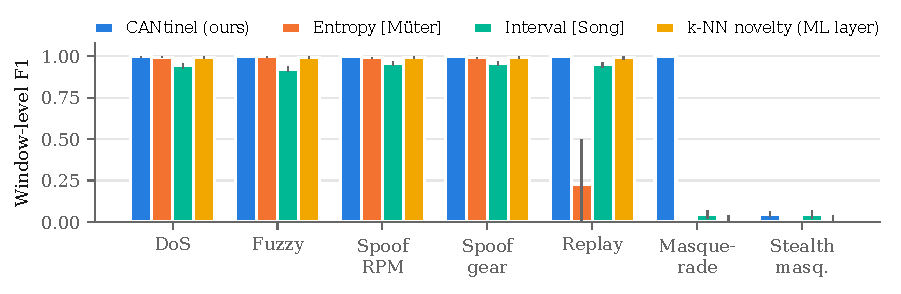
\includegraphics[width=\linewidth]{figures/fig_window_f1.pdf}
\caption{Window-level F1 (100\,ms windows, mean $\pm$ std over 5 vehicles).}\label{fig:window}
\end{figure}

\textbf{Window level} (Fig.~\ref{fig:window}). Entropy and k-NN handle floods but fail on masquerade (F1
$<$0.02) and, for entropy, on replay (0.22); CANtinel is best on every attack except the stealth masquerade. L4 changed F1
by about 0.01 at most but raised the clean-window FPR to 0.6\,\%, so it is optional.

\begin{table}[t]
\centering
\begin{minipage}[t]{0.44\linewidth}
\centering
\caption{Ablation, frame F1 (+L2: L1 with timing; +L3: L1 with payload).}\label{tab:ablation}
\scriptsize
\begin{tabular}{@{}lcccc@{}}
\toprule
Attack & L1 & +L2 & +L3 & All\\
\midrule
DoS & 1.000 & 1.000 & 1.000 & 1.000\\
Fuzzy & 0.994 & 0.994 & 1.000 & 1.000\\
Spoof RPM & 0.000 & 0.941 & 0.800 & 0.991\\
Spoof gear & 0.000 & 0.902 & 0.761 & 0.964\\
Replay & 0.000 & 1.000 & 1.000 & 1.000\\
Masquerade & 0.000 & 0.004 & 0.999 & 0.999\\
Stealth masq. & 0.000 & 0.004 & 0.000 & 0.004\\
\bottomrule
\end{tabular}

\end{minipage}\hfill
\begin{minipage}[t]{0.53\linewidth}
\centering
\caption{SecOC-lite: PDUs accepted by the receiver.}\label{tab:secoc}
\scriptsize
\begin{tabular}{@{}lr@{}}
\toprule
Scenario & Accepted / sent\\
\midrule
Legitimate PDUs & 3{,}000 / 3{,}000\\
Legitimate, 10\,\% frame loss & 2{,}691 / 2{,}691\\
Replay of sniffed PDUs & 0 / 500\\
Spoofing, random MAC & 0 / 1{,}000\\
Stealth masq., re-used trailer & 0 / 1{,}000\\
Stealth masq., guessed FV & 0 / 1{,}000\\
MAC brute force (one PDU) & 0 / 200{,}000\\
\bottomrule
\end{tabular}

\end{minipage}
\end{table}

\textbf{Ablation} (Table~\ref{tab:ablation}). Timing is essential for spoofing, payload semantics for masquerade,
either catches replay, and for spoofing their fusion beats either layer alone because payload-invalid frames can no longer capture
the timing anchor.

\begin{figure}[t]
\centering
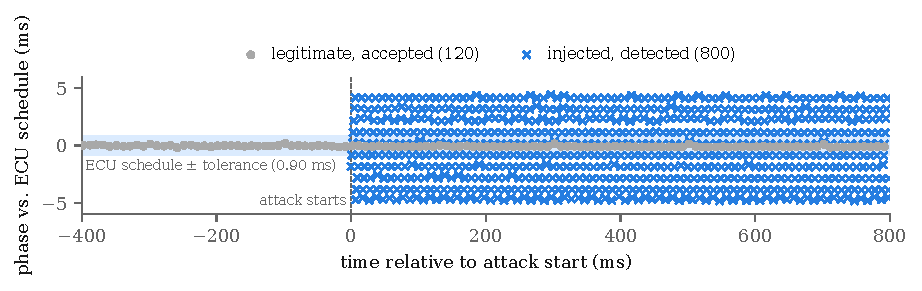
\includegraphics[width=\linewidth]{figures/fig_phase.pdf}
\caption{Phase-locked timing during a typical gear-spoofing burst (ID 0x43F): genuine frames stay on the ECU's schedule,
injected frames arrive at every phase and are rejected.}\label{fig:phase}
\end{figure}

\textbf{Explainability} (Fig.~\ref{fig:phase}). A typical alert reads \emph{``0x4B0 CHECKSUM\_FAIL: byte 7: crc8 checksum 0x64 $\neq$ expected 0xBA''}, which an
analyst can check directly.

\textbf{Prevention.} The gateway blocked 96.4--100\,\% of the frames of every detectable attack while forwarding at
least 99.2\,\% of genuine frames. SecOC-lite (Table~\ref{tab:secoc}) accepted every genuine PDU, even with 10\,\% loss,
and rejected all replayed, forged and stealth-masquerade PDUs and all 200{,}000 brute-force guesses.

\textbf{Performance.} The engine processes about 196{,}000 frames/s on one core in pure Python, over 40 times the
maximum rate of a full 500\,kbit/s bus; a SecOC-lite MAC costs about 2\,\textmu s.

% ---------------------------------------------------------------------
\section{Discussion and Conclusion}
% ---------------------------------------------------------------------
Unlike the tools in Table~\ref{tab:market}, CANtinel is auditable (every rule is a JSON entry, every alert carries
evidence), needs no DBC files or labelled attacks, couples detection with prevention and authentication, runs on
commodity hardware for fleets and start-ups facing AIS-189, and is tested on masquerade attacks~\cite{verma2024road}.

\textbf{Limitations.} Results come from a simulator, not a vehicle; validation on HCRL, ROAD and a test bench is
next. Spoofed values that are legal successors remain partly ambiguous, stealth masquerades need authentication and
key provisioning, and electrical evidence~\cite{longari2025canter,cho2016cids} is not yet used.

\textbf{Conclusion.} CAN's missing access control, authenticity and freshness let one node starve most of a vehicle's
messages or override safety-relevant signals. CANtinel detects flooding, spoofing, replay and naive masquerade
attacks with F1 0.96--1.00 at an FPR of $2.3\times10^{-6}$, explains every alert, and its SecOC-lite layer stops the
stealth masquerade no anomaly detector can see. Future work: a C port, CAN~FD/Ethernet support and test-bench validation.

\bibliographystyle{splncs04}
\bibliography{references}

\end{document}
